\documentclass{beamer}
\usepackage{amsmath, amssymb, amsthm}
\usepackage{graphicx, fancyhdr}

% Theme choice
\usetheme{metropolis} % Modern and clean layout

% Footer settings
\setbeamertemplate{footline}{
  \leavevmode\hbox{\begin{beamercolorbox}[wd=\paperwidth,ht=3ex,dp=2ex]{author in head/foot}%
      \hspace{1em} {M. J. Moghaddas Mehr}
      \, \textbar \,
      \insertshorttitle \,
      \textbullet \, 
      \insertsection \, 
      \hfill \insertframenumber{}/\inserttotalframenumber{} \hspace{.5em}
  \end{beamercolorbox}
  }
}

% Title Page Details
\title{Isomorphism in Union-Closed Sets}
\author{Mohammad Javad Moghaddas Mehr}
\date{Cincinnati – March 2025}


\begin{document}

% Title Slide
\begin{frame}
	\titlepage
\end{frame}

% Outline Slide
\begin{frame}{Outline}
	\begin{figure}\label{fig:lattice_with_rank}
		\centering
		% First diagram
		\begin{minipage}{0.45\textwidth}
			\centering
			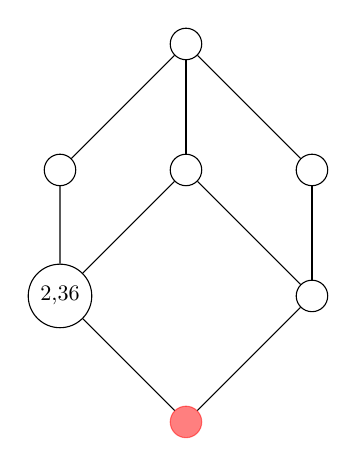
\begin{tikzpicture}[scale=.8, transform shape, every node/.style={draw, circle, minimum size=0.5cm}]
				% Nodes
				\node[fill=red, opacity=0.5, draw=red] (empty) at (0, 0) {};
				\node (x) at (-2, 2) {2,36};
				\node (z) at (2, 2) {};
				\node (xy) at (-2, 4) {};
				\node (xz) at (0, 4) {};
				\node (yz) at (2, 4) {};
				\node (xyz) at (0, 6) {};

				% Edges
				\draw (empty) -- (x);
				\draw (empty) -- (z);
				\draw (x) -- (xy);
				\draw (x) -- (xz);
				\draw (z) -- (xz);
				\draw (z) -- (yz);
				\draw (xy) -- (xyz);
				\draw (xz) -- (xyz);
				\draw (yz) -- (xyz);
			\end{tikzpicture}
		\end{minipage}
		\hfill
		% Second diagram
		\begin{minipage}{0.45\textwidth}
			\centering
			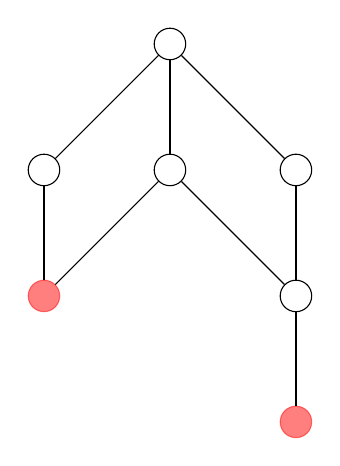
\begin{tikzpicture}[scale=.8, transform shape, every node/.style={draw, circle, minimum size=0.5cm}]
				% Nodes
				\node[fill=red, opacity=0.5, draw=red] (y) at (2, 0) {};
				\node[fill=red, opacity=0.5, draw=red] (x) at (-2, 2) {};
				\node (z) at (2, 2) {};
				\node (xy) at (-2, 4) {};
				\node (xz) at (0, 4) {};
				\node (yz) at (2, 4) {};
				\node (xyz) at (0, 6) {};

				% Edges
				\draw (y) -- (z);
				\draw (x) -- (xy);
				\draw (x) -- (xz);
				\draw (z) -- (xz);
				\draw (z) -- (yz);
				\draw (xy) -- (xyz);
				\draw (xz) -- (xyz);
				\draw (yz) -- (xyz);
			\end{tikzpicture}
		\end{minipage}
		\caption{Two lattice diagrams. The red nodes belong to \(\mathcal{K}^{\bot}\).}
	\end{figure}
\end{frame}

% Introduction Slide
\section{Introduction}
\begin{frame}{Introduction}
	\begin{itemize}
		\item Definition of Union-Closed Families of Sets
		\item Péter Frankl's Union-Closed Set Conjecture
		\item Our Focus: Structural Properties of Isomorphisms
	\end{itemize}
\end{frame}

% Definitions Slide
\section{Definitions and Theorems}
\begin{frame}{Definitions}
	\textbf{Union-Closed Family:} A collection $\mathcal{K} \subseteq 2^{[n]}$ is union-closed if for all $A, B \in \mathcal{K}$, we have $A \cup B \in \mathcal{K}$.

	\vspace{1em}
	\textbf{Isomorphism:} A bijection $h: \mathcal{K}_1 \to \mathcal{K}_2$ such that:
	\begin{equation*}
		h(A \cup B) = h(A) \cup h(B) \quad \forall A, B \in \mathcal{K}_1.
	\end{equation*}
\end{frame}

% Main Theorem Slide
\begin{frame}{Main Theorem}
	\textbf{Theorem:} For every isomorphism $h: \mathcal{K}_1 \to \mathcal{K}_2$, there exists a corresponding hyperisomorphism $H: \bigcup \mathcal{K}_1 \to \bigcup \mathcal{K}_2$ such that:
	\begin{equation*}
		h(A) = \{H(a) \mid a \in A\}, \quad \forall A \in \mathcal{K}_1.
	\end{equation*}
\end{frame}

% Conclusion Slide
\section{Conclusion}
\begin{frame}{Conclusion}
	\begin{itemize}
		\item Structural preservation under isomorphisms
		\item Connection to the Union-Closed Set Conjecture
		\item Future work: applications of hyperisomorphisms
	\end{itemize}
\end{frame}

% Thank You Slide
\begin{frame}
	\centering
	{\Huge \textbf{Thank You!}}
	\\ Questions?
\end{frame}

\end{document}
